\documentclass[a4paper, 11pt, oneside]{article}
\usepackage[doublespacing]{setspace}
\usepackage[scale=0.75]{geometry}
\usepackage[affil-it]{authblk}
\usepackage{enumerate}
\usepackage{hyperref}
\usepackage{amsmath}
\usepackage{algorithm}
\usepackage{graphicx}
\usepackage{csquotes}
\usepackage[noend]{algpseudocode}
\graphicspath{ {../latex_figures/} }
\usepackage{booktabs,tabularx}
    \newcolumntype{L}{>{\raggedright\arraybackslash}X}
\usepackage{graphicx}
\usepackage{amssymb}

\makeatletter
\def\BState{\State\hskip-\ALG@thistlm}
\makeatother

\title{Review of Multiple Comparison Correction methods\\
	\Large - From the Bonferroni procedure to Efron's Local FDR - }
\author{2014140089 Park, Si Hyung}
%\affil{Division of Life Sciences, Korea University}
%\date{}

\begin{document}
\maketitle

\section{Introduction}
    Ever since works on multiple comparison problem (MCP) were started by Tukey (1949) and Scheff\'e (1953), who have both utilized $t-$statistic for pairwise sample mean comparisons, numerous procedures for controlling family-wise error rate (FWER) have been developed. Achieving higher testing power while controlling FWER for the same level has especially been a major concern in the field of MCP, rulling the field for almost 35 years before Benjamini and Hochberg suggested the concept of false discovery rate (FDR) in 1995. \par
    In this brief report, I would like to review two major concepts in MCP - FWER, FDR - and some of the selected procedures which control FWER or FDR in certain level. Historical meanings and important proofs were described to better highlight modifications and developments of a statistical concept over time. Keep in mind that many of the proofs written in this review were simplified to achieve intuitive delivery of the concept. Simple simulation of multiple testing was also conducted to compare different methods of MCP correction.

\subsection{Multiple comparison problem}
Multiple comparison problem (MCP), also known as multiple hypothesis tesing problem or multiplicity problem, is a problem which occurs when a family-level hypothesis testing is made based on a set of individual hypotheses. Due to the fact that a family-level type I error rate (family-wise error rate; FWER) is always greater than an experiment-level type I error ($\because 1-(1-\alpha)^m > \alpha,$ if $m \geq 2$), an appropriate correction for the error control of family-level hypothesis testing is needed.

\subsection{Adjusted p-values}
Adjusted p-values are the values that are calculated from original p-values. We can compare adjusted p-values with the level which we control family-level error for. For example, if an adjusted p-value of a hypothesis $H_i$ is less than or equal to $\alpha_0$, then we can reject $H_i$ while controlling $FWER$ for $\alpha_0$. Unlike p-values, adjusted p-values do not give us the information about the type I error probability of that hypothesis.

\subsection{Regression dependency of hypotheses}
For some family-level error controlling procedure, assumption on dependence structure is needed. Let $I_0$ be a subset of indices of hypotheses in a set of tests. If there exists no regression dependence between non-rejected test statistics and true-null test statistics, then the hypotheses in a set are said to be independent. If there is a positive regression dependence between non-rejected test statistics and true-null test statistics, then the hypotheses in the set are said to have positive regression dependency on each one from a subset $I_0$ ($PRDS$ on $I_0$). Benjamini and Yekutieli (2001) defined $PRDS$ on $I_0$ as follows: \enquote{For any increasing set $D$, and for each $i \in I_0$, $P(X \in D | X_i = x)$ is non-decreasing in $x$}. More intuitive explanation uses p-values. For each $i \in I_0$, If p-values increases, then probability that corresponding null hypothesis is true does not decreases.

\subsection{Notations}
\begin{table}[ht]
    \small
    \setlength{\tabcolsep}{3pt}
\centering
\begin{tabularx}{.7\hsize}{@{}l LLL@{}}
    \toprule
 & Declared as non-significant  & Declared as significant & Total \\
    \midrule
True $H_0$ 
    & $U$ 
        & $V$ 
            & $m_0$ \\
False $H_0$ 
    & $T$ 
        & $S$
            &  $m_1=m-m_0$ \\
Total & $m-R$ 
        & $R$ 
            & $m$ \\
    \bottomrule
\end{tabularx}
\caption{notation of the number of hypotheses in corresponding to each cell}
    \end{table}

Notations used to define family-level error concepts mathematically are as described on Table 1. This notation follows that of Benjamini and Hochberg (1995). Total $m$ hypotheses in a set is being tested in this situation. $m_0 \leq m$ hypotheses are true null. Note that $R$, the number of rejected hypotheses, is an observable random variable while $U$, $V$, $T$, $S$ are unobservable random variables.
\vspace{0.2in}


\section{Family-Wise Error Rate (FWER)}
Family-wise error rate is a probability that at least one of the type I error occurs when testing each individual hypothesis in a set. Using previous notations, it can be defined as $P(V \geq 1) = 1 - P(V=0) = E(I_{V \geq 1})$. If FWER is controlled at level $\alpha_0$, then probability that one or more type I error occurs in the set is less than or equal to $\alpha_0$. \par
    In early works, FWER was controlled by using a specific type of test statistic - $t$, normal, multivariate $t$, or multivariate normal. After Bonferroni procedure was introduced, precedures using p-values from individual testings became dominant.

\subsection{Bonferroni procedure}
Bonferroni procedure, widely used nowadays, was suggested by Dunn (1961). Dunn originally suggested a method to construct confidence interval in MCP using Bonferroni's inequality, which the procedure was named after. By testing individual hypotheses on level $\alpha/m$, we can control FWER at level $\alpha$. We can prove this with Boole's inequality (1).

\begin{equation}
\begin{aligned}\label{proof-bonf}
&\text{By Boole's inequality }P(\cup_{i=1}^{n}E_i)\leq\sum_{i=1}^n P(E_i),\\
& FWER=P(\cup_{i=1}^{m_0}(p_i\leq\dfrac{\alpha}{m}))\leq\sum_{i=1}^{m_0}P(p_i\leq\dfrac{\alpha}{m})=m_0\dfrac{\alpha}m\leq\alpha
\end{aligned}
\end{equation}

Adjusted (or \enquote{Bonferronied}) p-value of $i$th hypothesis is equal to $min(p_i \times m, 1)$.

\begin{algorithm}
\caption{Bonferroni Procedure}\label{bonf}
\begin{algorithmic}[1]
\Procedure{Bonferroni}{}
\State $\textit{pvals} \gets \text{array of p-values}$
\State $\textit{adj\_pvals} \gets \text{empty array of length same as } \textit{pvals}$
\BState \text{\textbf{For} \textit{i} in 1:\textit{length(pvals})}:
\State {$adj\_pvals[i] \gets pvals[i] * length(pvals)$}
\If {$adj\_pvals[i] \leq \alpha$} {reject $i$th hypothesis}
\EndIf
\EndProcedure
\end{algorithmic}
\end{algorithm}

Dunn simplified MCP correction in two major ways. (i) Dunn introduced a control procedure which is based on individual p-values. It is possible to conduct any kind of multiple testing, even it does not use specific type of test statistic. (ii) Bonferroni procedure is remarkably computationally efficient. By setting the procedure as \textit{algorithm 1}, Bonferroni correction only costs $O(n)$. In many big-data analyses where high complexity algorithms are not feasible to use, Bonferroni procedure can help. Also, Bonferroni procedure does not require the assumption of regression dependence. However, excessive loss in testing power in Bonferroni procedure led to the development of stepwise FWER controlling procedures.

\subsection{Holm procedure}
In addition to improve power of test while controlling for same level of FWER, Holm (1979) designed a step-up procedure. In fact, it is one of the first stepwise algorithm for MCP correction. Holm procedure can be conducted as follows. 
\begin{enumerate}
  \item Sort p-values in increasing order: $p_{(1)}, p_{(2)}, ..., p_{(m)}$.
    \begin{enumerate}[-]
    \item Each of the p-value corresponds to $H_{0_{(1)}}, H_{0_{(2)}}, ..., H_{0_{(m)}}$. 
    \end{enumerate}
  \item Find the smallest $j$, in which $p_{(j)} > \dfrac{\alpha}{m-j+1}$.
  \item Reject $H_{0_{(k)}}$'s, where $k=1, 2, ..., (j-1)$.
\end{enumerate}

By rejecting hypotheses with Holm procedure, we can control FDR for level $\alpha_0$ (2).

\begin{equation}
\begin{aligned}\label{proof-bonf}
& \text{If the smallest index which satisfies } p_{(j)} > \dfrac{\alpha}{m-j+1} \text{ is } j \text{, then} \\
& m-j+1 \geq m_0,\text{ } \dfrac{1}{m-j+1} \leq \dfrac{1}{m_0} \text{,  }
p_{(j-1)} \leq \dfrac{\alpha}{m-j+2} \leq \dfrac{\alpha}{m_0}.\\
& \therefore \text{By Boole's inequality, } FWER=P(\cup_{i=1}^{m_0}(p_i\leq\dfrac{\alpha}{m_0}))\leq\sum_{i=1}^{m_0}P(p_i\leq\dfrac{\alpha}{m_0})=\alpha\\
\end{aligned}
\end{equation}

Adjusted p-value of $i$th hypothesis for Holm procedure is equal to $min(p_i \times (m-i+1), 1)$. \par
    As Holm procedure compares individual p-values to $\dfrac{\alpha}{m}, \dfrac{\alpha}{m-1}, ..., \dfrac{\alpha}{1}$ instead of uniform level $\dfrac{\alpha}{m}$ as in Bonferroni procedure, Holm procedure is uniformly more powerful than Bonferroni procedure, though the power gain is little. Holm procedure also does not assume specific regression dependence of hypotheses.


\subsection{Hochberg procedure}
Hochberg (1988) sharpened Holm's method to be more powerful. In his two-paged paper, he modified Holm procedure and suggested step-up algorithm with similar rejection critetion. 
\begin{enumerate}
  \item Sort p-values in increasing order: $p_{(1)}, p_{(2)}, ..., p_{(m)}$.
  \item Find the largest $j$, in which $p_{(j)} \leq \dfrac{\alpha}{m-j+1}$.
  \item Reject $H_{0_{(k)}}$'s, where $k=1, 2, ..., j$.
\end{enumerate}
    With a little modification, Hochberg procedure is uniformly more powerful than Holm procedure. However, this algorithm requires non-negative regression dependence assumption to properly control FWER at certain level. Although testing power increase in Hochberg procedure is almost negligible, it later inspired Hochberg to develop a step-up FDR controlling procedure.

\vspace{0.2in}


\section{False Discovery Rate (FDR)}
While the field concentrated on improving testing power of FWER controlling method, some insisted to develop a new concept of family-level error, other than FWER. FWER has drawbacks: (i) Controlling for FWER has much less power than controlling for experiment-wise error. (ii) In many cases it is not necessary to control FWER in strong manner made. Saville is the one who recommended using per comparison error rate (PCER) than FWER, because of these reasons. \par
    Inspired by the fact that the ratio of the number of false rejection to the number of total rejection might be a useful error rate to control for, Benjamini and Hochberg (1995) introduced a seminal concept, false discovery rate (FDR). FDR is defined as \enquote{the expectation of the ratio of the number of erroneous rejection to the number of total rejection}, which can be denoted as $E(Q)=E(V/R)=E(V/(S+V))$. By defining FDR as $E(Q)$, relationship with FWER can be derived.
    \begin{enumerate}
    \item if $m_0=m$, then FDR $=$ FWER. \\
      $\because s=0$, $v=r$. $P(V \geq 1)= E(Q)$
    \item if $m_0<m$, then FDR $\leq$ FWER. \\
      $\because v>0$, $Q \leq I_{V \geq 1}$, $E(Q) \leq E(I_{V \geq 1}) = P(V \geq 1)$
    \end{enumerate}
Because of this relationship, controlling for FWER also controls FDR in strong manner. In contrary, controlling for FDR weakly controls FWER (does not assure that FWER is also being controlled). \par
    Due to the high testing power, it is recommended to use FDR in following cases. (i) When the family-level conclusion is insensitive to failures in individual testing. (ii) When conducting exploratory analysis, or screening to find as many potential discoveries as possible.

\subsection{Benjamini-Hochberg (B-H) procedure}
Alongside the introduction of FDR, Benjamini and Hochberg developed a step-up procedure to easily control FDR at certain level $q^*$.
\begin{enumerate}
  \item Sort p-values in increasing order: $p_{(1)}, p_{(2)}, ..., p_{(m)}$.
  \item Find the largest $j$, in which $p_{(j)} \leq \dfrac{j}{m}q^*$.
  \item Reject $H_{0_{(k)}}$'s, where $k=1, 2, ..., j$.
\end{enumerate}
Unlike the Hochberg procedure for FWER control which used hyperbolic form of constant ($\dfrac{\alpha}{m-\textbf{\textit{j}}+1}$), the B-H procedure for FDR control uses linear form of constant ($\dfrac{\textbf{\textit{j}}}{m}q^*$). Because linear form of constant shrinks slowly than that of hyperbolic form, the B-H procedure has much larger testing power than that of FWER controlling procedures. Benjamini and Hochberg suggested that the procedure would work properly under independence assumption. It was later proved to be appropriate method under PRDS too (Benjamini and Yekutieli, 2001) (3), (4).


\subsection{Benjamini-Yekutieli (B-Y) procedure}
Benjamini and Yekutieli introduced a modified version of the B-H procedure, which can handle the situation under arbitrary dependency. By comparing ordered p-value $p_{(j)}$ to $\dfrac{j}{m \cdot c(m)}q^*$ (under non-negative dependece $c(m)=1$ otherwise $=\sum_{j=1}^m \dfrac{1}{j}$), instead of $\dfrac{j}{m \cdot c(m)}q^*$, the B-Y procedure can control FDR at desired level even under negative or arbitrary regression dependence (3), (5).

\begin{equation}
\begin{aligned}\label{proof-by1}
& \text{Let } C_{v, s}^{(i)} \text{ be the event in which if } p_i \text{ is rejected then } (v-1) \text{ true nulls and \textit{s} false nulls}\\
& \text{are rejected alongside with it. Then we can define } C_k^{(i)}=\cup \{C_{v,s}^{(i)} \text{: } v+s=k \} \text{ and } \\
& FDR=E(Q)=\sum_{i=1}^{m_0} \sum_{k=1}^m \dfrac{1}{k}P(p_i \leq q_k \cap C_k^{(i)}).\\
\end{aligned}
\end{equation}

\begin{equation}
\begin{aligned}\label{proof-by2}
\text{Under PRDS, } E(Q)&=\sum_{i=1}^{m_0} \sum_{k=1}^m \dfrac{1}{k}P(p_i \leq q_k \cap C_k^{(i)}) \leq \sum_{i=1}^{m_0} \sum_{k=1}^m \dfrac{q^*}{m} \dfrac{P(p_i \leq q_k \cap C_k^{(i)})}{P(p_i \leq q_k)}\\
& \leq \sum_{i=1}^{m_0} \dfrac{q^*}{m} \cdot 1 = m_0 \dfrac{q}{m} \leq q^*
\end{aligned}
\end{equation}

\begin{equation}
\begin{aligned}\label{proof-by3}
\text{Under arbitraty} &\text{ dependence, define } p_{ijk}=P(\{ p_i \in [\dfrac{j-1}{m}q^*, \dfrac{j}{m}q^*]\} \cap C_k^{(i)}). \text{ Then}\\ 
E(Q)&=\sum_{i=1}^{m_0} \sum_{k=1}^m \dfrac{1}{k}P(p_i \leq q_k \cap C_k^{(i)}) = \sum_{i=1}^{m_0} \sum_{k=1}^{m} \dfrac{1}{k} \sum_{j=1}^{k} p_{ijk}\\
& = \sum_{i=1}^{m_0} \sum_{j=1}^{m} \sum_{k=j}^{m} \dfrac{1}{k}p_{ijk} \leq \sum_{i=1}^{m_0} \sum_{j=1}^{m} \sum_{k=j}^{m} \dfrac{1}{j}p_{ijk} \\
& \leq \sum_{i=1}^{m_0} \sum_{j=1}^{m} \dfrac{1}{j} \sum_{k=1}^{m} p_{ijk} = m_0 \sum_{j=1}^{m} \dfrac{1}{j} \dfrac{q^*}{m} \leq \sum_{j=1}^m \dfrac{1}{j} q^*
\end{aligned}
\end{equation}

\subsection{Brief introduction to local FDR}
While control procedure for family-level of FDR has been developed, nothing described an expected false rejection ratio of an individual hypothesis in the set. FDR controlling procedures utilized experiment-wise p-values, which were probability of the type I error, not the expected rate of false rejection. \par
    To report the expected false rejection rate of individual gene of interest from microarray data, Efron (2001) grafted empirical bayes approach to MCP. In empricial bayes method, hyperparameters of prior distribution are fitted using the observed data, unlike standard bayes method which sets hyperparameters beside the data. Efron defined local-level of FDR (local FDR) as $fdr(z)=\dfrac{p_0 f_0(z)}{f(z)}$, where $z$ is the domain of the densities (observed data), $p_0$ is a prior probability that a hypothesis (null) is true, $f_0(Z)$ is the density of true nulls, $f_1(Z)$ is the density of false nulls, and $f(Z)=p_0f_0(Z) + p_1f_1(Z)$ is the joint density of true and false nulls, which can be expressed as a mixture of true and false null densities. For crude local FDR inference in large sample, we can use $p_0 \geq 0.9$, $f_0(Z) \stackrel{d}{=} N(0, 1)$, and estimate $f(Z)$ with $Poisson$ GLM.

\vspace{0.2in}


\section{Discussions - Simulation and Comparisons}
A simple simulation was conducted to compare different kinds of MCP correction procedures. Two FWER methods (Bonferroni, Holm) and Benjamini-Hochberg FDR method, Efron's local FDR method were compared. Experiment-level p-values were compared to Efron's local FDR. Simulation scheme is as described:
\begin{enumerate}
  \item Total 2,000 random samples were generated. 1,000 samples were generated from $N(0, 1)$, and 1,000 other samples were generated from $N(3, 1)$.
  \item p-values were calculated by two-sided $Z$-testing each sample (sample size were set to one in each Z-test).
 \item Adjusted p-values or local FDR were calculated to compare procedures at equal family-level error. Graphical description of adjusted p-values were generated.
\end{enumerate}

\begin{figure}[ht]
\centering
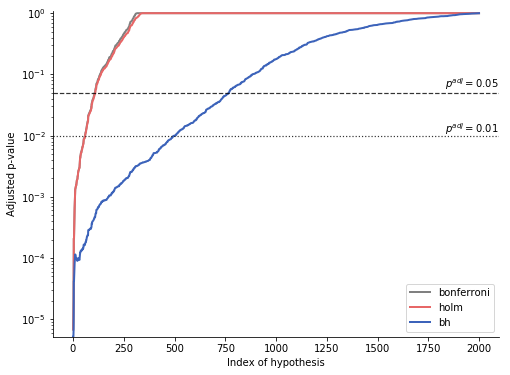
\includegraphics[scale=0.4]{adj_pval_report} 
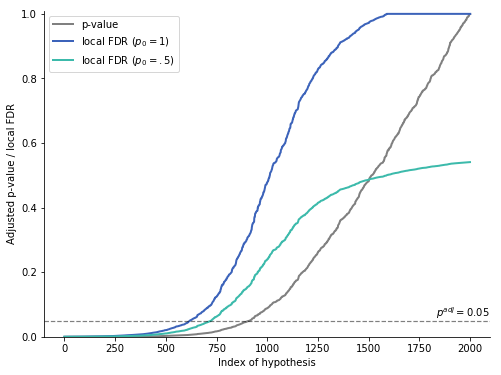
\includegraphics[scale=0.4]{pval-lfdr_report}
\caption{simple Z-test simulation for comparison of MCP correction methods}
\end{figure}

Controlling for FDR has much more power gain than Bonferroni or Holm FWER method (Figure 1, left). While only \~{}110 rejections were made in FWER controlling procedures, 739 rejections were made in the B-H FDR procedure. Ratios of false rejection to total rejection were .009, .009, .014 respectively, suggesting that the B-H procedure appropriately controlled FDR in desired manner. \par
    Local FDRs have generally higher value than corresponding p-values (Figure 1, right), indicating that the expected false rejection rate in an interval which contains a hypothesis of interest is usually larger than the type I error rate. While the difference was quite large, it is possible to lower the values of local FDR by accurately estimating $p_0$. With $p_0=0.5$, the result was much more reasonable in this generated dataset, considering the correspondence to individual p-values.

\pagebreak

\section{References}
\setstretch{1}
 Holm, S. (1979). "A Simple Sequentially Rejective Multiple Test Procedure". Scandinavian Journal of Statistics, 6(2), 65-70 \vspace{0.06in}\\
 Abdi, H. (2010). "Holm's Sequential Bonferroni Procedure". University of Texas at Dallas \vspace{0.06in}\\
 Aickin, M., Gensler, H. (1996). "Adjusting for multiple testing when reporting research results: the Bonferroni vs Holm methods". American Journal of Public Health, 86(5), 726-728 \vspace{0.06in}\\
 Benjamini, Y., Hochberg, Y. (1995). "Controlling the False Discovery Rate: A Practical and Powerful Approach to Multiple Testing". Journal of the Royal Statistical Society. Series B (Methodological), 57(1), 289-300 \vspace{0.06in}\\
 Benjamini, Y., Yekutieli, D. (2001). "The control of the false discovery rate in multiple testing under dependency". Ann. Statist. 29(4), 1165-1188 \vspace{0.06in}\\
 Robinson, D. (2015). "Understanding empirical Bayes estimation (using baseball statistics)". From \href{http://varianceexplained.org/r/empirical\_bayes\_baseball/}{Variance Explained}, retrieved at Dec. 2017 \vspace{0.06in}\\
 Efron, B., Tibshirani, R., Storey, J., Tusher, V. (2001). "Empirical Bayes Analysis of a Microarray Experiment". Stanford University Technical Report. 216 \vspace{0.06in}\\
 Efron, B. (2005). "Local False Discovery Rates". Stanford University Technical Report. 234 \vspace{0.06in}\\




\end{document}  